\documentclass{beamer}
\usetheme{metropolis}

\usepackage{graphicx}

\usepackage{mathtools}
\usepackage{amssymb}
\usepackage{mathabx}
\usepackage[all]{xy}

\title{Combinatorial Species}
\subtitle{A tool for the perplexed mathematical biologist}

\date{\today}
\author{Egor Lappo}
\institute{Rosenberg Lab}

\begin{document}
\maketitle
\section{motivation}

\begin{frame}{(perfectly plausible) problems}
  \begin{itemize}
    \item \textbf{Tanglegrams.} How many tanglegrams are there for your set of species? \pause What if trifurcations are allowed? \pause $k$-furcations? \pause
    \item \textbf{Allele identity configurations.} For $n$ individuals with $k$ alleles at a locus, how many identity states are there? \pause What if individuals are distinguishable? \pause
    \item \textbf{Monkeys.} Each of the $n$ monkeys gives a fruit to another monkey. How many exchange configurations need to be considered? \pause What if monkeys can't give fruits to themselves? \pause What if there are blue monkeys and red monkeys?
  \end{itemize}
\end{frame}

\begin{frame}{what is the \emph{first} thing you do?}
  \pause
  \begin{itemize}
    \item \textbf{Compute.} \pause
    \item \textbf{Guess.} \pause
    \item \textbf{Write proofs.} \pause
    \item Try out the combinatorial species approach!
  \end{itemize}
\end{frame}

\section{definition}

\begin{frame}{definition}
  \begin{definition}
    A \textbf{species of structures} is a rule $F$ that
    \begin{itemize}
      \item for each finite set $U$ gives a finite set $F[U]$,
      \item for each bijection $U\to V$ gives a function $F[U] \to F[V]$,
      \item respects composition.
    \end{itemize}
  \end{definition} \pause
  \begin{example}
    Species $\mathcal A$ of rooted trees, $\mathcal G$ of simple graphs, $\mathcal S$ of permutations, $\mathrm{Par}$ of partitions, etc.
  \end{example} \pause
  The juice of the theory is in the \emph{combinators} of species and \emph{associated series}.
\end{frame}

\begin{frame}{definition}

  $U$, $V$ are finite sets, $\sigma$ is a bijection.

  \[
    \xymatrix{U \ar[dd]_\sigma \ar[r] &  F[U] \ar[dd]^{F[\sigma]} \\ & \\
    V \ar[r] &  F[V]}
  \] \pause

  $F[\sigma]$ is \emph{not} necessarily a bijection.

\end{frame}

\begin{frame}{species of rooted trees}
  \begin{center}
    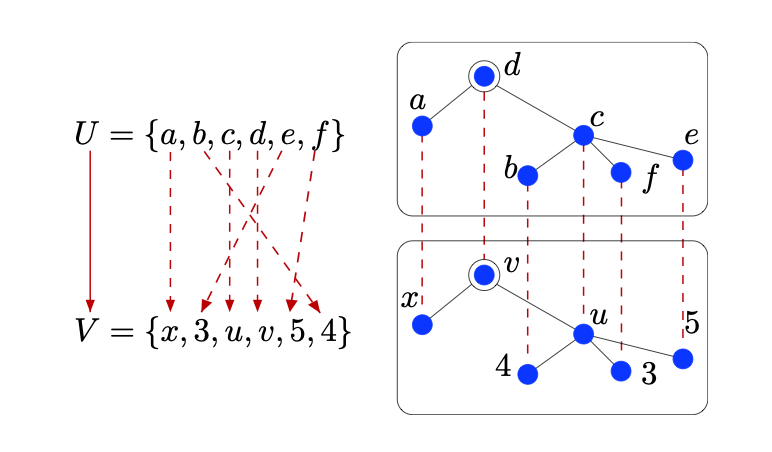
\includegraphics[width=10.5cm]{figures/tree_aut.png}
  \end{center}
\end{frame}

\begin{frame}{species of simple graphs}
  \begin{center}
    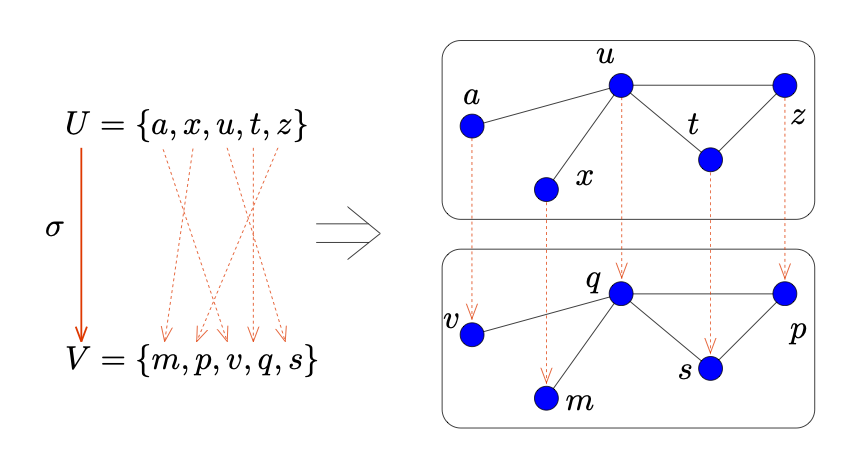
\includegraphics[width=10.5cm]{figures/graph_aut.png}
  \end{center}
\end{frame}

\begin{frame}{key aspects}
  \begin{itemize}
    \item Several basic constructions --- building blocks
    \item Combinators --- generalizing generating functions
    \item Associated series --- enumeration
    \item Functional equations, Lagrange inversion, virtual species, \ldots
  \end{itemize}
\end{frame}

\begin{frame}{basic species: sets}
  Species of sets $E$: $E[U] = \{U\}$.

  \[
    \xymatrix{U \ar[r] \ar[d]_\sigma & E[U] = \{U\} \ar[d]^{E[\sigma]} \\ V \ar[r] & E[V] = \{\sigma(U)\}}
  \]

  Unique choice for each $U$.
\end{frame}

\begin{frame}{basic species: sets}
  Species of elements $\varepsilon$: $\varepsilon[U] = U$.

  \[
    \xymatrix{U \ar[r] \ar[d]_\sigma & \varepsilon[U] = U \ar[d]^{\varepsilon[\sigma]=\sigma} \\ V \ar[r] & \varepsilon[V] = V}
  \]

  Kind of identity.
\end{frame}

\begin{frame}{basic species: specific cardinality}
  \begin{itemize}
    \item Species $1$, characteristic of the empty set, with
          \[
            1[U] = \begin{cases} \{U\}, & \text{if $U = \emptyset$}\\ \emptyset, & \text{otherwise.}\end{cases}
          \] \pause
    \item Species $X$, characteristic of singletons, with
          \[
            X[U] = \begin{cases} \{U\}, & \text{if $|U| = 1$}\\ \emptyset, & \text{otherwise.}\end{cases}
          \] \pause
    \item Species $E_2$ of pairs, etc.
  \end{itemize}
\end{frame}

\section{the part where is all pays off}

\begin{frame}{associated series I}
  \begin{definition}
    Let $F$ be a species. The \textbf{cycle index series} of $F$ is the formal power series
    \[
      Z_F(x_1, x_2, x_3, \ldots) = \sum_{n=0}^\infty \frac{1}{n!} \left(\sum_{\sigma \in \mathcal S_n} \mathrm{fix}\, F[\sigma]\, x_1^{\sigma_1} x_2^{\sigma_2} x_3^{\sigma_3}\cdots\right),
    \]
    where $\sigma$ are all permutations of $[n]$, $\mathrm{fix}\,F[\sigma]$ is the number of fixed points of $F[\sigma]$, and $\sigma_i$ is the number of cycles of $\sigma$ of length $i$.
  \end{definition}\pause
  This contains \emph{all} information on the enumeration of $F$.
\end{frame}

\begin{frame}{example}
  Let $F[n]$ be the species of rooted trees on $n$ leaves.
  \[
    F[3] = \big\{a = ((1,2),3), b=((2,3),1), c = ((3,1),2)\big\}
  \]
  Let $\sigma = \{1,2,3\} \to \{1,3,2\}$. We have $\sigma_1 = 1$, $\sigma_2 = 1$.

  Then $F[3](a) = b$, $F[3](b) = a$, $F[3](c) = c$, so that $\mathrm{fix}\,F[\sigma] = 1$.
\end{frame}

\begin{frame}{associated series II}

  Let $F(x)$ be the exponential generating function for $F$, counting labeled $F$-structures,
  \[
    F(x) = \sum_{n=0}^\infty |F[n]| \frac{x^n}{n!}.
  \]

  Let $\widetilde{F}(x)$ be the generating function enumerating \textbf{unlabeled} $F$-structures,
  \[
    \widetilde{F(x)} = \sum_{n=0}^\infty \widetilde{f_n} x^n.
  \]
\end{frame}

\begin{frame}{associated series III}

  \begin{theorem}
    For any species $F$, we have
    \begin{align*}
      F(x)             & = Z_F(x,0,0,\ldots),     \\
      \widetilde{F(x)} & = Z_F(x,x^2,x^3,\ldots).
    \end{align*}
  \end{theorem} \pause

  Combinations of species correspond to operations on $Z_F$.
\end{frame}

\section{what are the combinators?}

\begin{frame}{combinators: sum}

  A \textbf{sum species} $F + G$ is a disjoint union. \pause

  \[|(F+G)[n]| = |F[n]| + |G[n]|, \]

  \[
    Z_{F+G} = Z_F + Z_G.
  \] \pause

  For example, $E = 1 + X + E_2 + E_3 + \cdots$.

\end{frame}

\begin{frame}{combinators: product}

  A \textbf{product species} $F\cdot G$ is an $F$- and a $G$- structure on two complementary disjoint subsets.

  For any finite set $U$,
  \[
    (F\cdot G)[U] = \sum_{\mathclap{(U_1,U_2)}} F[U_1] \times G[U_2].
  \] \pause

  \[
    Z_{F\cdot G} = Z_F\, Z_G
  \]

\end{frame}

\begin{frame}{combinators: product}
  \begin{center}
    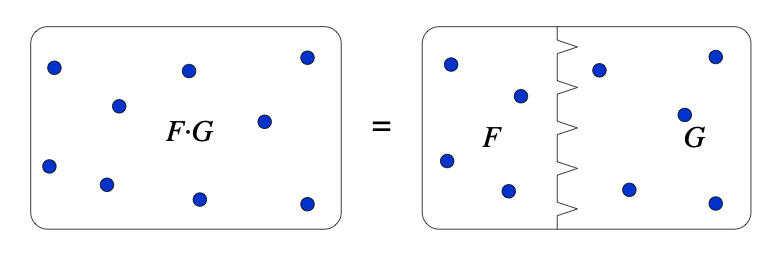
\includegraphics[width=10.5cm]{figures/product.png}
  \end{center}
\end{frame}

\begin{frame}{combinators: product}
  A permutation is a set of fixed points together with a derangement.

  \[
    \mathcal S = E\cdot \mathrm{Der}.
  \]

  \begin{center}
    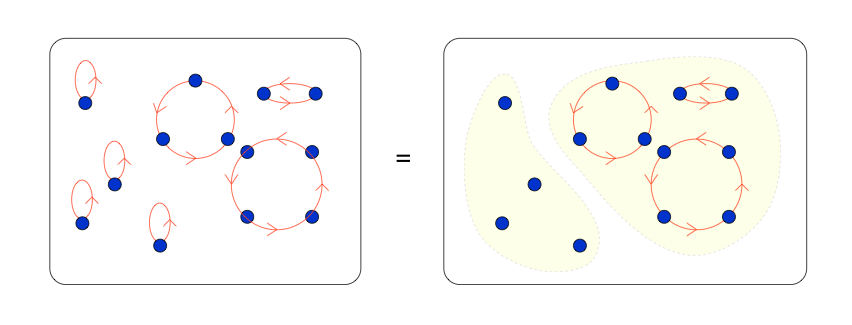
\includegraphics[width=10.5cm]{figures/permutation.png}
  \end{center}
\end{frame}

\begin{frame}{combinators: substitution}
  Finally, a composite species $F\circ G$ represents an $F$-assembly of disjoint $G$-structures. \pause

  For any finite set $U$,
  \[
    (F\circ G)[U] = \sum_{\text{$\pi$ partition of $U$}} F[\pi] \times \prod_{p\in \pi} G[p].
  \] \pause

  For the associated series, we have
  \begin{align*}
    Z_{F\circ G}(x_1,x_2,x_3,\ldots) & = Z_F(Z_G(x_1,x_2,x_3,\ldots),Z_G(x_2,x_4,\ldots),\ldots,             \\
    \widetilde{(F\circ G)(x)}        & = Z_F(\widetilde{G(x)}, \widetilde{G(x^2)},\widetilde{G(x^3)},\ldots) \\
    (F\circ G)(x)                    & = F(G(x))
  \end{align*} \pause

  Note that we can't do this unlabeled enumeration without the cycle index series.

\end{frame}

\begin{frame}{combinators: substitution}
  \begin{center}
    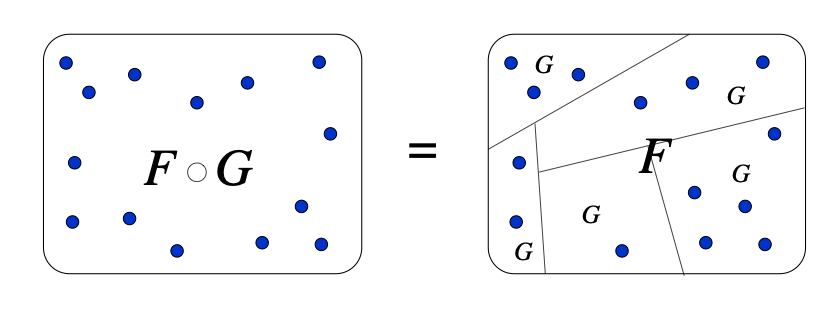
\includegraphics[width=10.5cm]{figures/substitution.png}
  \end{center}
\end{frame}

\begin{frame}{combinators: substitution}
  An endofunction is a permutation of trees,

  \[
    \mathrm{End} = \mathcal S \circ \mathcal A = \mathcal S(\mathcal A).
  \]

  \begin{center}
    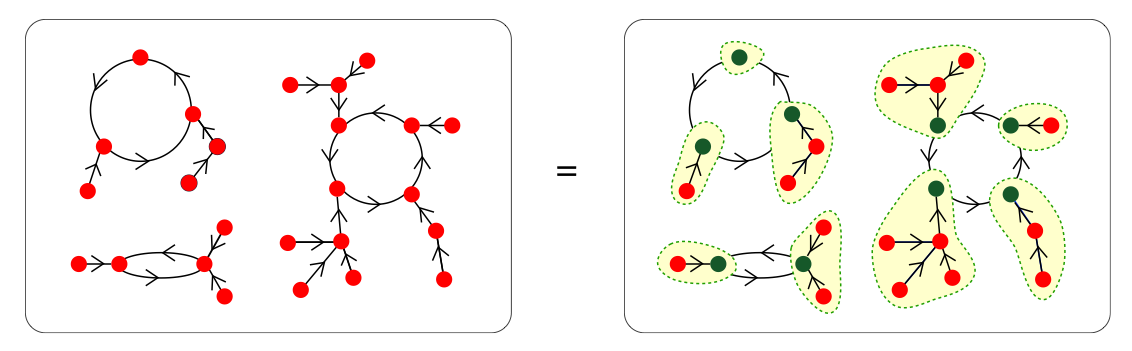
\includegraphics[width=10.5cm]{figures/endofunction.png}
  \end{center}
\end{frame}

\begin{frame}{summary}
Combinatorial species is a \emph{language}. \pause 

What else is there?
\begin{itemize}
  \item Species derivatives
  \item Weighted species, multisort species
  \item Virtual species
  \item Lagrange inversion to solve $Y = H(X,Y)$
  \item \textbf{Computer code}
\end{itemize}
\end{frame}

\end{document}